



\subsection{2.6. Диаграммы МО гомоатомных и гетероатомных двухатомных молекул (молекулярных ионов) для описания химических и магнитных свойств. Дипольный момент молекулы.} 

\par\bigskip
	
	С помощью диаграмм МО можно определить, является ли
	молекула или ион парамагнитной или диамагнитной, её порядок и
	кратность связи а также то, чем оно является: кислотой или
	основанием Льюиса.
	
	\par\smallskip
	
	Диаграммы МО для гомоатомных молекул (молекулярных ионов)
	симметричны, поскольку по обеим сторонам диаграммы
	располагаются атомы с одинаковыми значениями
	электроотрицательности.
	
	\par\smallskip
	
	Рассмотрим МО для гомоатомных молекул на примере 2 периода:
	
	
	
	\begin{figure}[H]
		\centering
		{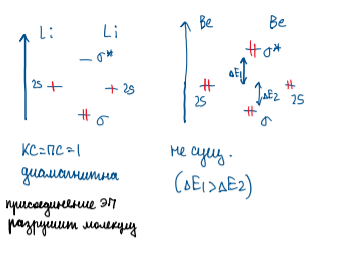
\includegraphics[scale=1]{15.png}}
	\end{figure}


\begin{figure}[H]
	\centering
	{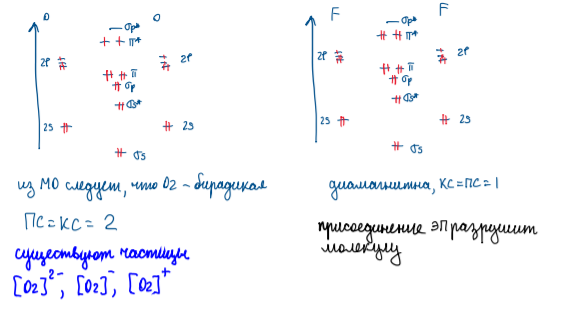
\includegraphics[scale=1]{16.png}}
\end{figure}
	
	\par\smallskip
	
	У $B_2, C_2, N_2$ МО выглядят подругому. Это связано с тем, что у
	них энергетические щели (то есть
	разделение по энергиям) между $s$- и
	$p$-орбиталями меньше. Сгустки
	электронной плотности
	оказываются очень близко и
	отталкиваются.
	
	
	\begin{figure}[H]
		\centering
		{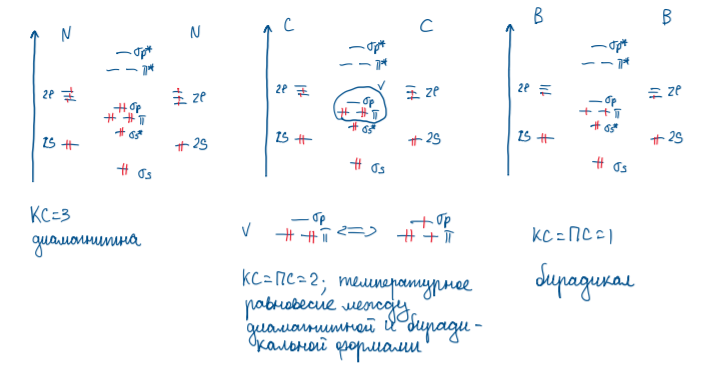
\includegraphics[scale=1]{17.png}}
	\end{figure}
	
	\par\smallskip
	
	Для гетероатомных систем диаграммы не будут симметричными,
	поскольку на них будут находиться атомы с разными значениями
	электроотрицательностями. Чем более электроотрицателен
	элемент, тем ниже по энергии он будет на диграмме. Здесь надо
	учитывать различие по энергии между перекрываемыми
	орбиталями: если оно слишком велико, перекрывание будет
	слабым, и наоборот. В остальном можно получить ту же
	информацию, что и для гомоатомных систем.
	
	\par\smallskip
	
	На примере $HF$:
	
	
	\begin{figure}[H]
		\centering
		{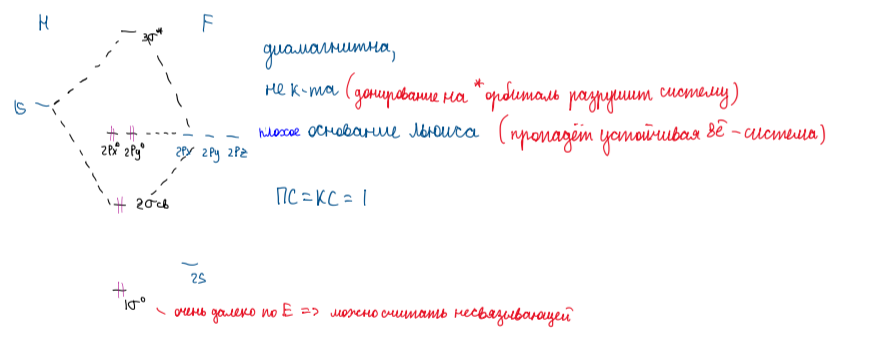
\includegraphics[scale=1]{18.png}}
	\end{figure}
	
	\par\smallskip
	
	Если требуется построить диаграмму МО для анионов
	предложенных молекул (если такие существуют), то надо добавить
	необходимое число электронов, начиная с самой низкой по энергии
	орбитали и двигаясь снизу вверх. Для катионов надо убрать
	необходимое число электронов с ВЗМО.
	
	\par\smallskip
	
	\begin{center}
\textbf{Дипольный момент молекулы.}			
	\end{center}

\par\smallskip
	
	Это физическая величина, которая позволяет оценить степень
	разделения зарядов в молекуле. Дипольный момент измеряется в
	Дебаях (Д). Для теоретической модели с полным разделением
	заряда, состоящей из одного протона и одного электрона,
	находящихся на расстоянии 1 Ангстрем, дипольный момент равен
	одному эпсилон-ангстрему (1 эпсилон-ангстрем = 4.803 Д). К слову,
	такая модель - единственное ионное «соединение», где разделение
	зарядов $100\%$-е.
	
	\par\smallskip
	
	С помощью дипольного момента молекулы можно оценить вклады
	ионной и ковалентной составляющих в связывание. Например, для
	молекулы воды в теоретических представлениях о полном
	разделении заряда дипольный момент составляет 1.18 еА, но
	экспериментальное значение - 0.387 еА. Следовательно, можно
	судить о том, что «ионности» у молекулы воды только примерно
	треть, а остальное приходится на «ковалентность».
	
	\par\smallskip
	
	Очевидно, что для гомоатомных систем дипольный момент равен
	нулю, потому что никакого смещения электронной плотности не
	происходит.


\par\bigskip
\par\bigskip
